\chapter{DESARROLLO DEL EXPERIMENTO}
\section{Construcción de los conjuntos finales de datos}
El conjunto total de datos utilizado para la investigación consistió en la recolección de 27,251 proyectos tecnológicos de Kickstarter comprendidos entre los años 2009 y 2019, en 3 partes: metainformación, descripción y comentarios (excluyendo los del creador) del proyectos.

\subsection{Metainformación}
Como se mencionó en las Técnicas de recolección de datos del Capítulo III, el punto de partida para la construcción de los conjuntos de datos fue consolidar las bases públicas, archivos de valores separados por comas (.csv) comprimidos, de la página Web Robots (https://webrobots.io/kickstarter-datasets/), fraccionadas por fechas mensuales de captura de información comenzadas desde noviembre del 2015 hasta agosto del 2019 (Figura \ref{4:fig1}), y posteriormente pre-procesada con la ayuda del software Alteryx Designer. De acuerdo con la información de los creadores del sitio Web Robots, se ejecutan robots en dos servidores en la nube encargados de recolectar en un determinado punto del día y una vez al mes información de las campañas que aparecen en Kickstarter \parencite{ot_webrobots2019kickstarter}.

\begin{figure}[!ht]
	\begin{center}
		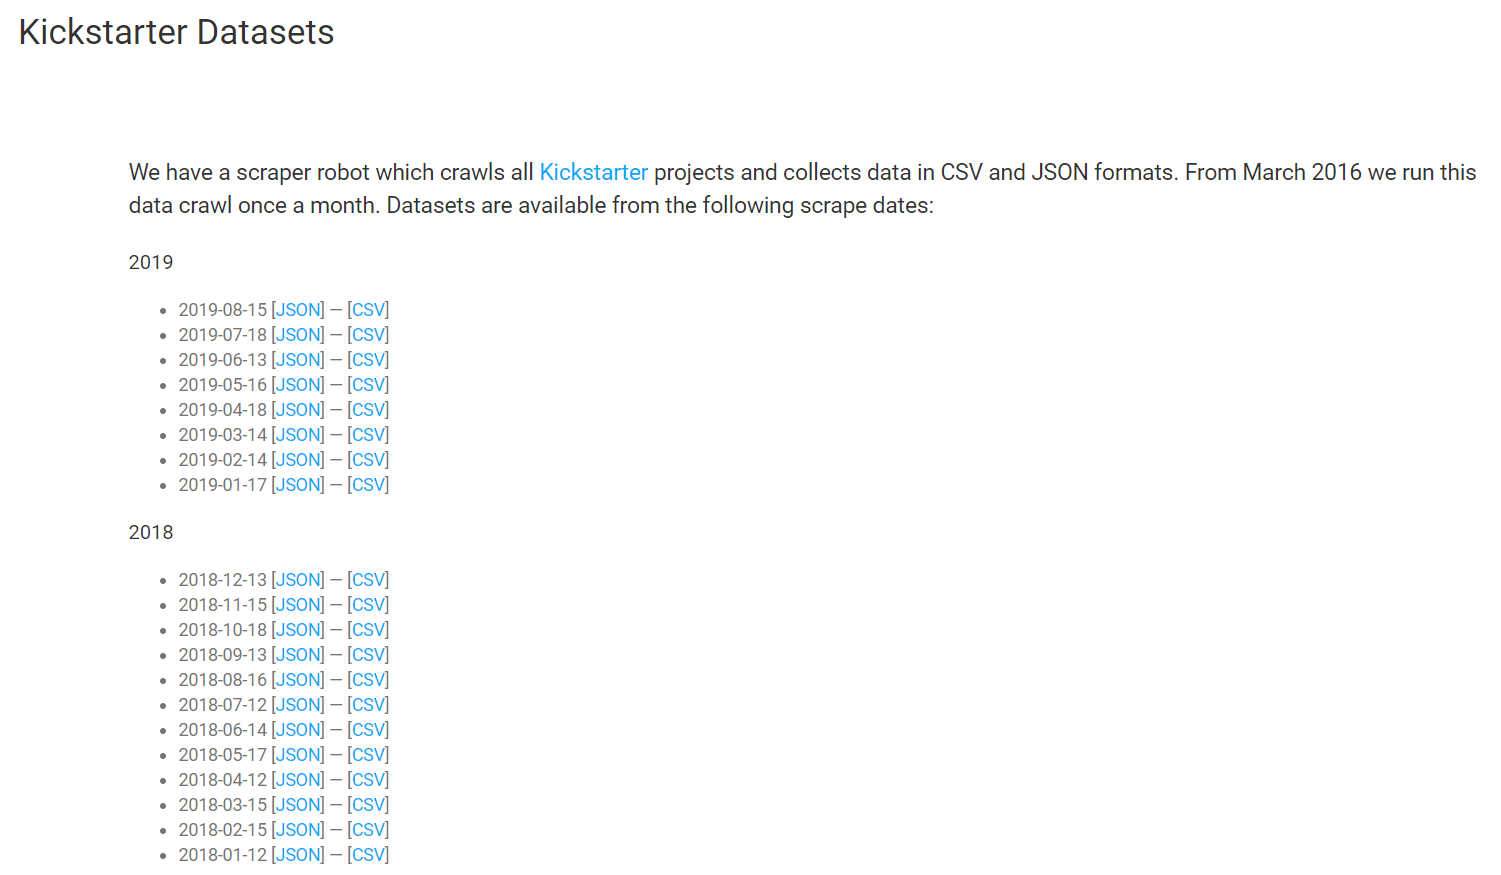
\includegraphics[width=0.8\textwidth]{4/figures/web_robots_2019.png}
		\caption{Vista (agosto 2019) del website Web Robots. Fuente: \cite{ot_webrobots2019kickstarter}}
		\label{4:fig1}
	\end{center}
\end{figure}

Cada archivo descargado por fecha de captura mensual es descomprimido, y las particiones en formato .csv que contienen son juntadas mediante el siguiente proceso:

\begin{itemize}
	\item Descargar librerías correspondientes de Python (pandas, numpy, glob, math).
	\item Dirigirse a la ruta de destino.
	\item Crear carpetas por mes para almacenar archivos particionados.
	\item Ejecutar algoritmo para unir archivos particionados csv dentro de una misma carpeta.
\end{itemize}

Cuando el algoritmo finaliza su ejecución, se crea un nuevo archivo separado por comas en cada carpeta por mes, cuyo tamaño oscila entre 1 y 5 gigabytes (GB) en total por cada uno. Con el fin de ahorrar espacio en memoria dentro de la computadora, los archivos particionados son eliminados y solamente se almacenan los nuevos generados.

Por ejemplo, en la Figura \ref{4:fig2} se detalla el tamaño del conjunto de datos total al corte del periodo de captura de información Julio 2019, aproximadamente más de 212 mil proyectos de todas las categorías y 37 columnas de variables.

\begin{figure}[h]
	\begin{center}
		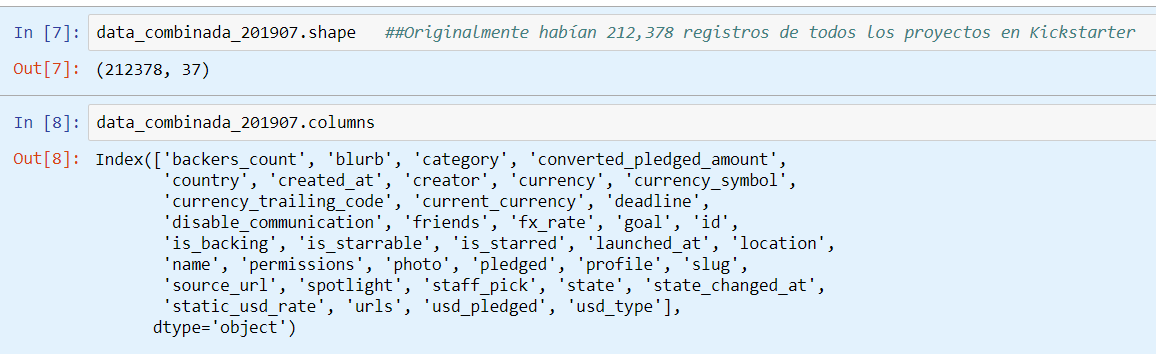
\includegraphics[width=0.9\textwidth]{4/figures/dataset_201907.png}
		\caption{Tamaño de conjunto de datos al corte de Julio 2019. Fuente: Elaboración propia.}
		\label{4:fig2}
	\end{center}
\end{figure}

A cada conjunto de datos generado se filtran los que pertenecen a la categoría \textit{\textbf{Technology}}. Debido a que no se cuenta con la información de la columna \textit{main\_category}, este proceso de filtración se logra utilizando la variable \textit{source\_url} al seleccionar aquellos registros que contengan la cadena de caracteres “https://www.kickstarter.com/discover/categories/technology”. En la Figura \ref{4:fig3} se aprecia cómo queda el conjunto filtrado por categoría Techonlogy al corte de Julio 2019.

\begin{figure}[h]
	\begin{center}
		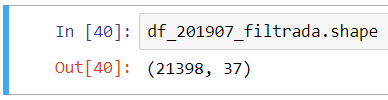
\includegraphics[width=0.5\textwidth]{4/figures/dataset_filtrada_201907.png}
		\caption{Tamaño de conjunto de datos filtrado del corte de Julio 2019. Fuente: Elaboración propia.}
		\label{4:fig3}
	\end{center}
\end{figure}

Cuando se repitió este procedimiento con cada conjunto de datos, se notó que la proporción de proyectos tecnológicos en Kickstarter representa el 10\% del total de proyectos. Esto se calculó al comparar los tamaños (cantidad de registros por fila) del conjunto de datos inicial y del filtrado.

La siguiente fase del pre-procesamiento fue la de seleccionar las variables de los nuevos conjuntos de datos filtrados que se usarán para generar el dataset final. Para ello, se usó el software Alteryx Designer, el cual permite desarrollar flujos de trabajo para preparar, unir y analizar volúmenes de datos complejos de distintas fuentes.

Con los conjuntos de datos filtrados, se creó el flujo de trabajo representado en la Figura \ref{4:fig4}.

\begin{figure}[htbp]
	\begin{center}
		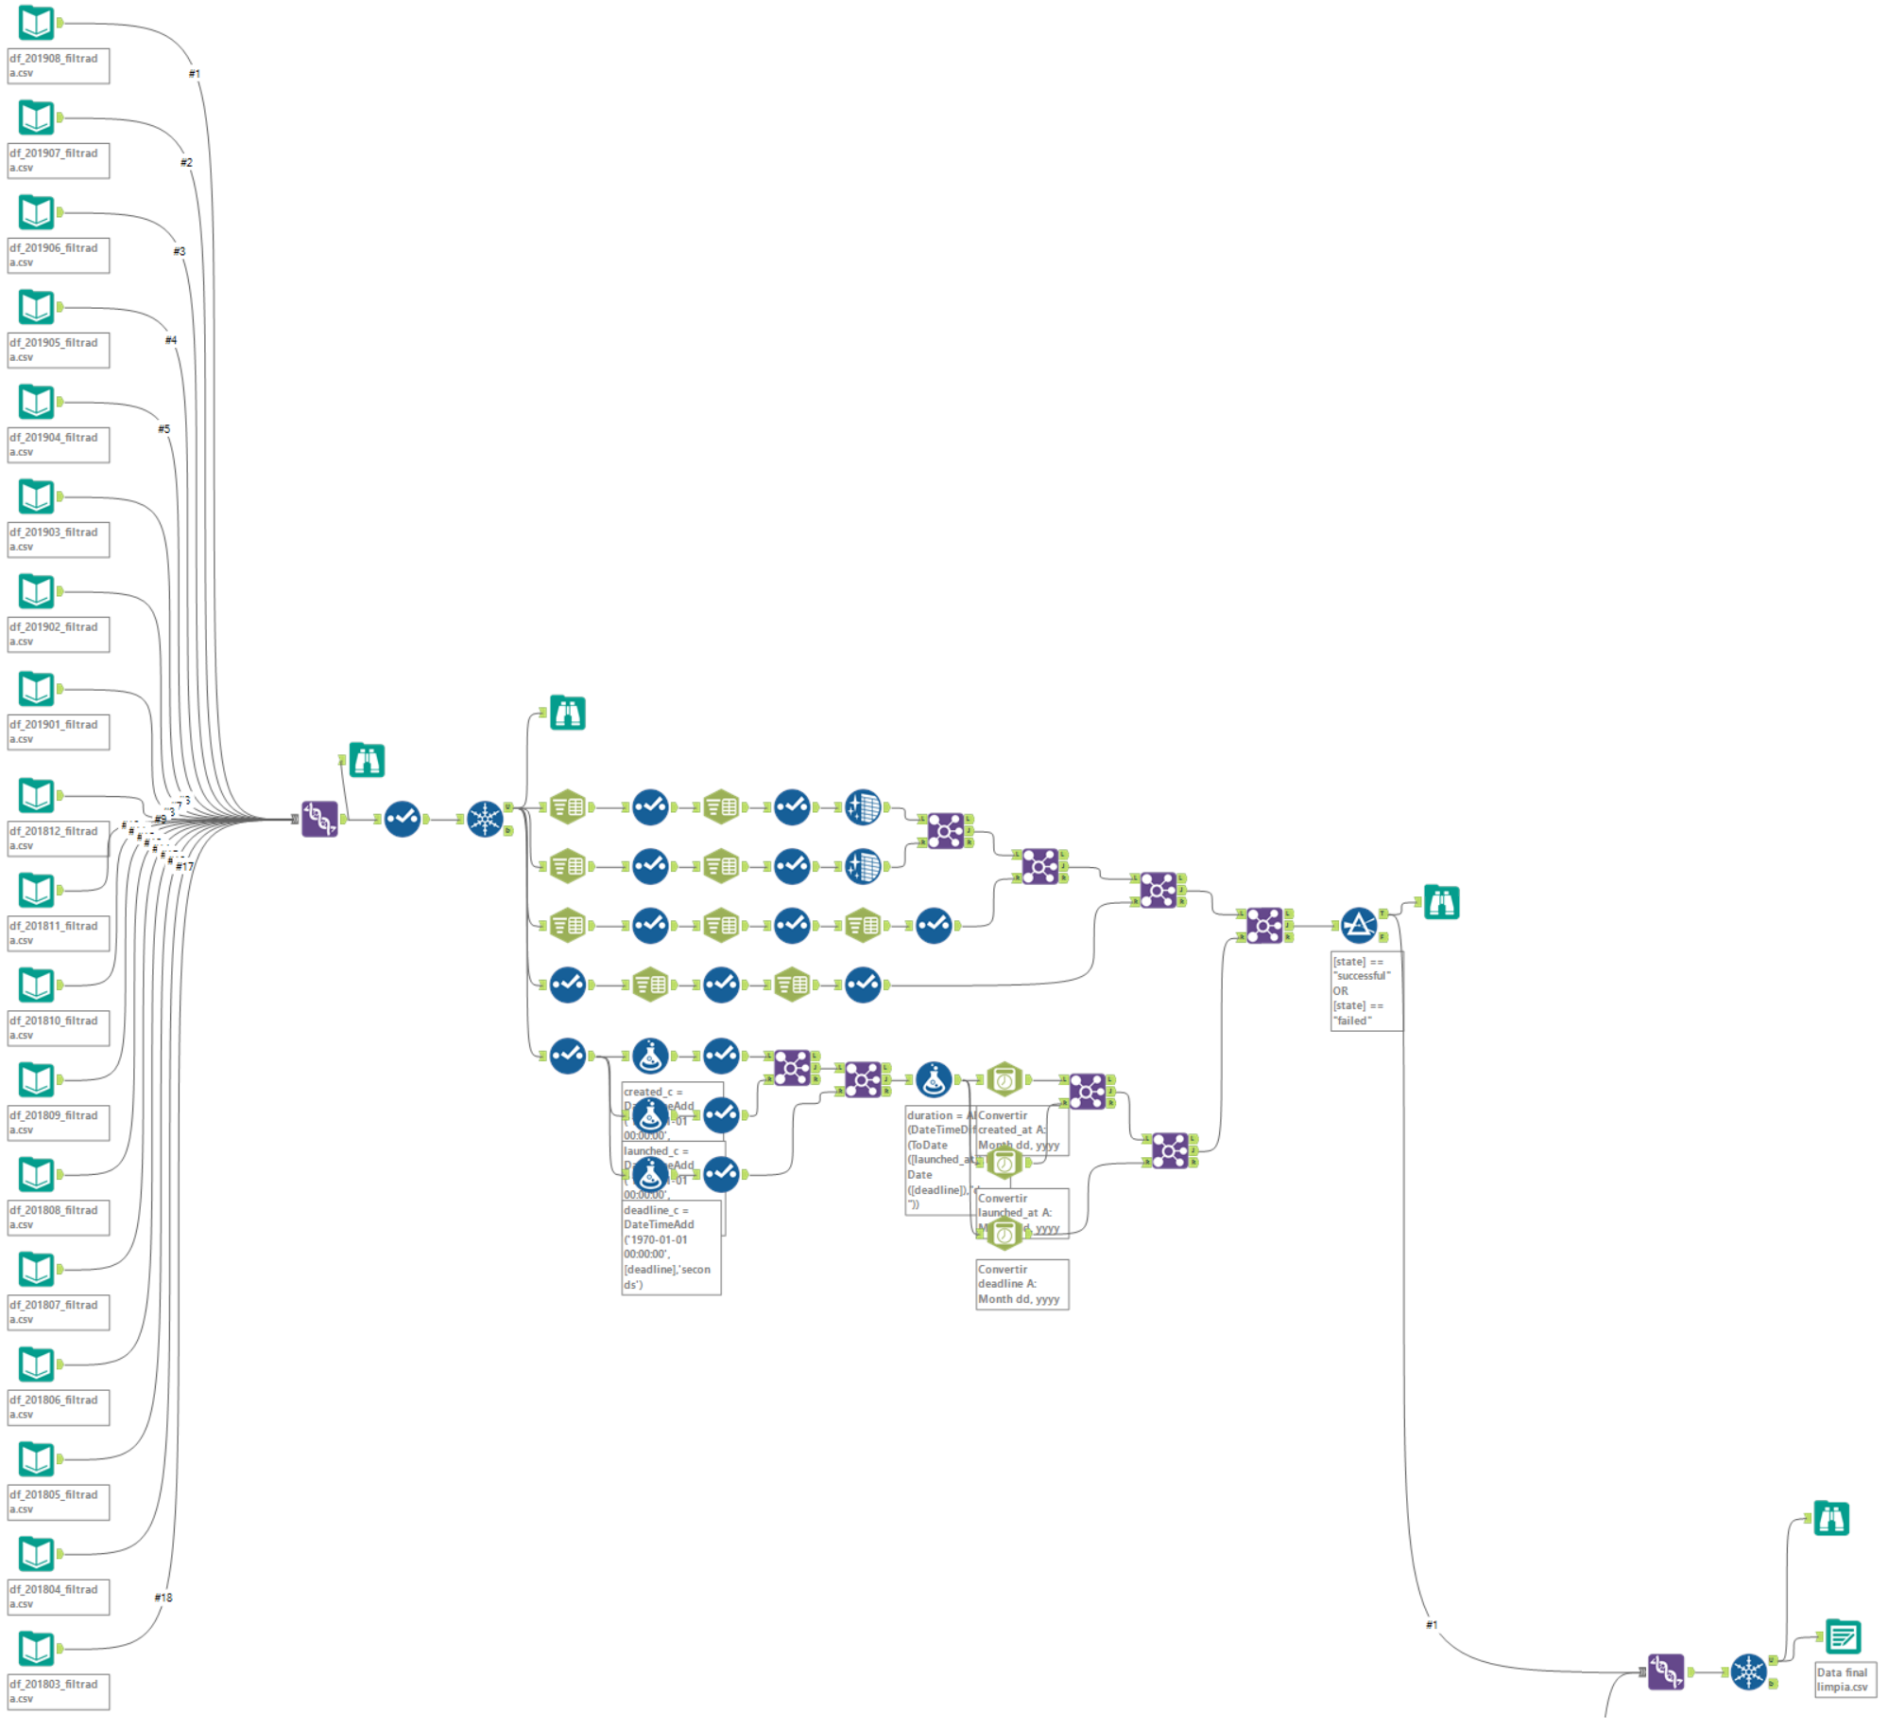
\includegraphics[width=0.7\textwidth]{4/figures/alteryx_flux_part1.png}	
		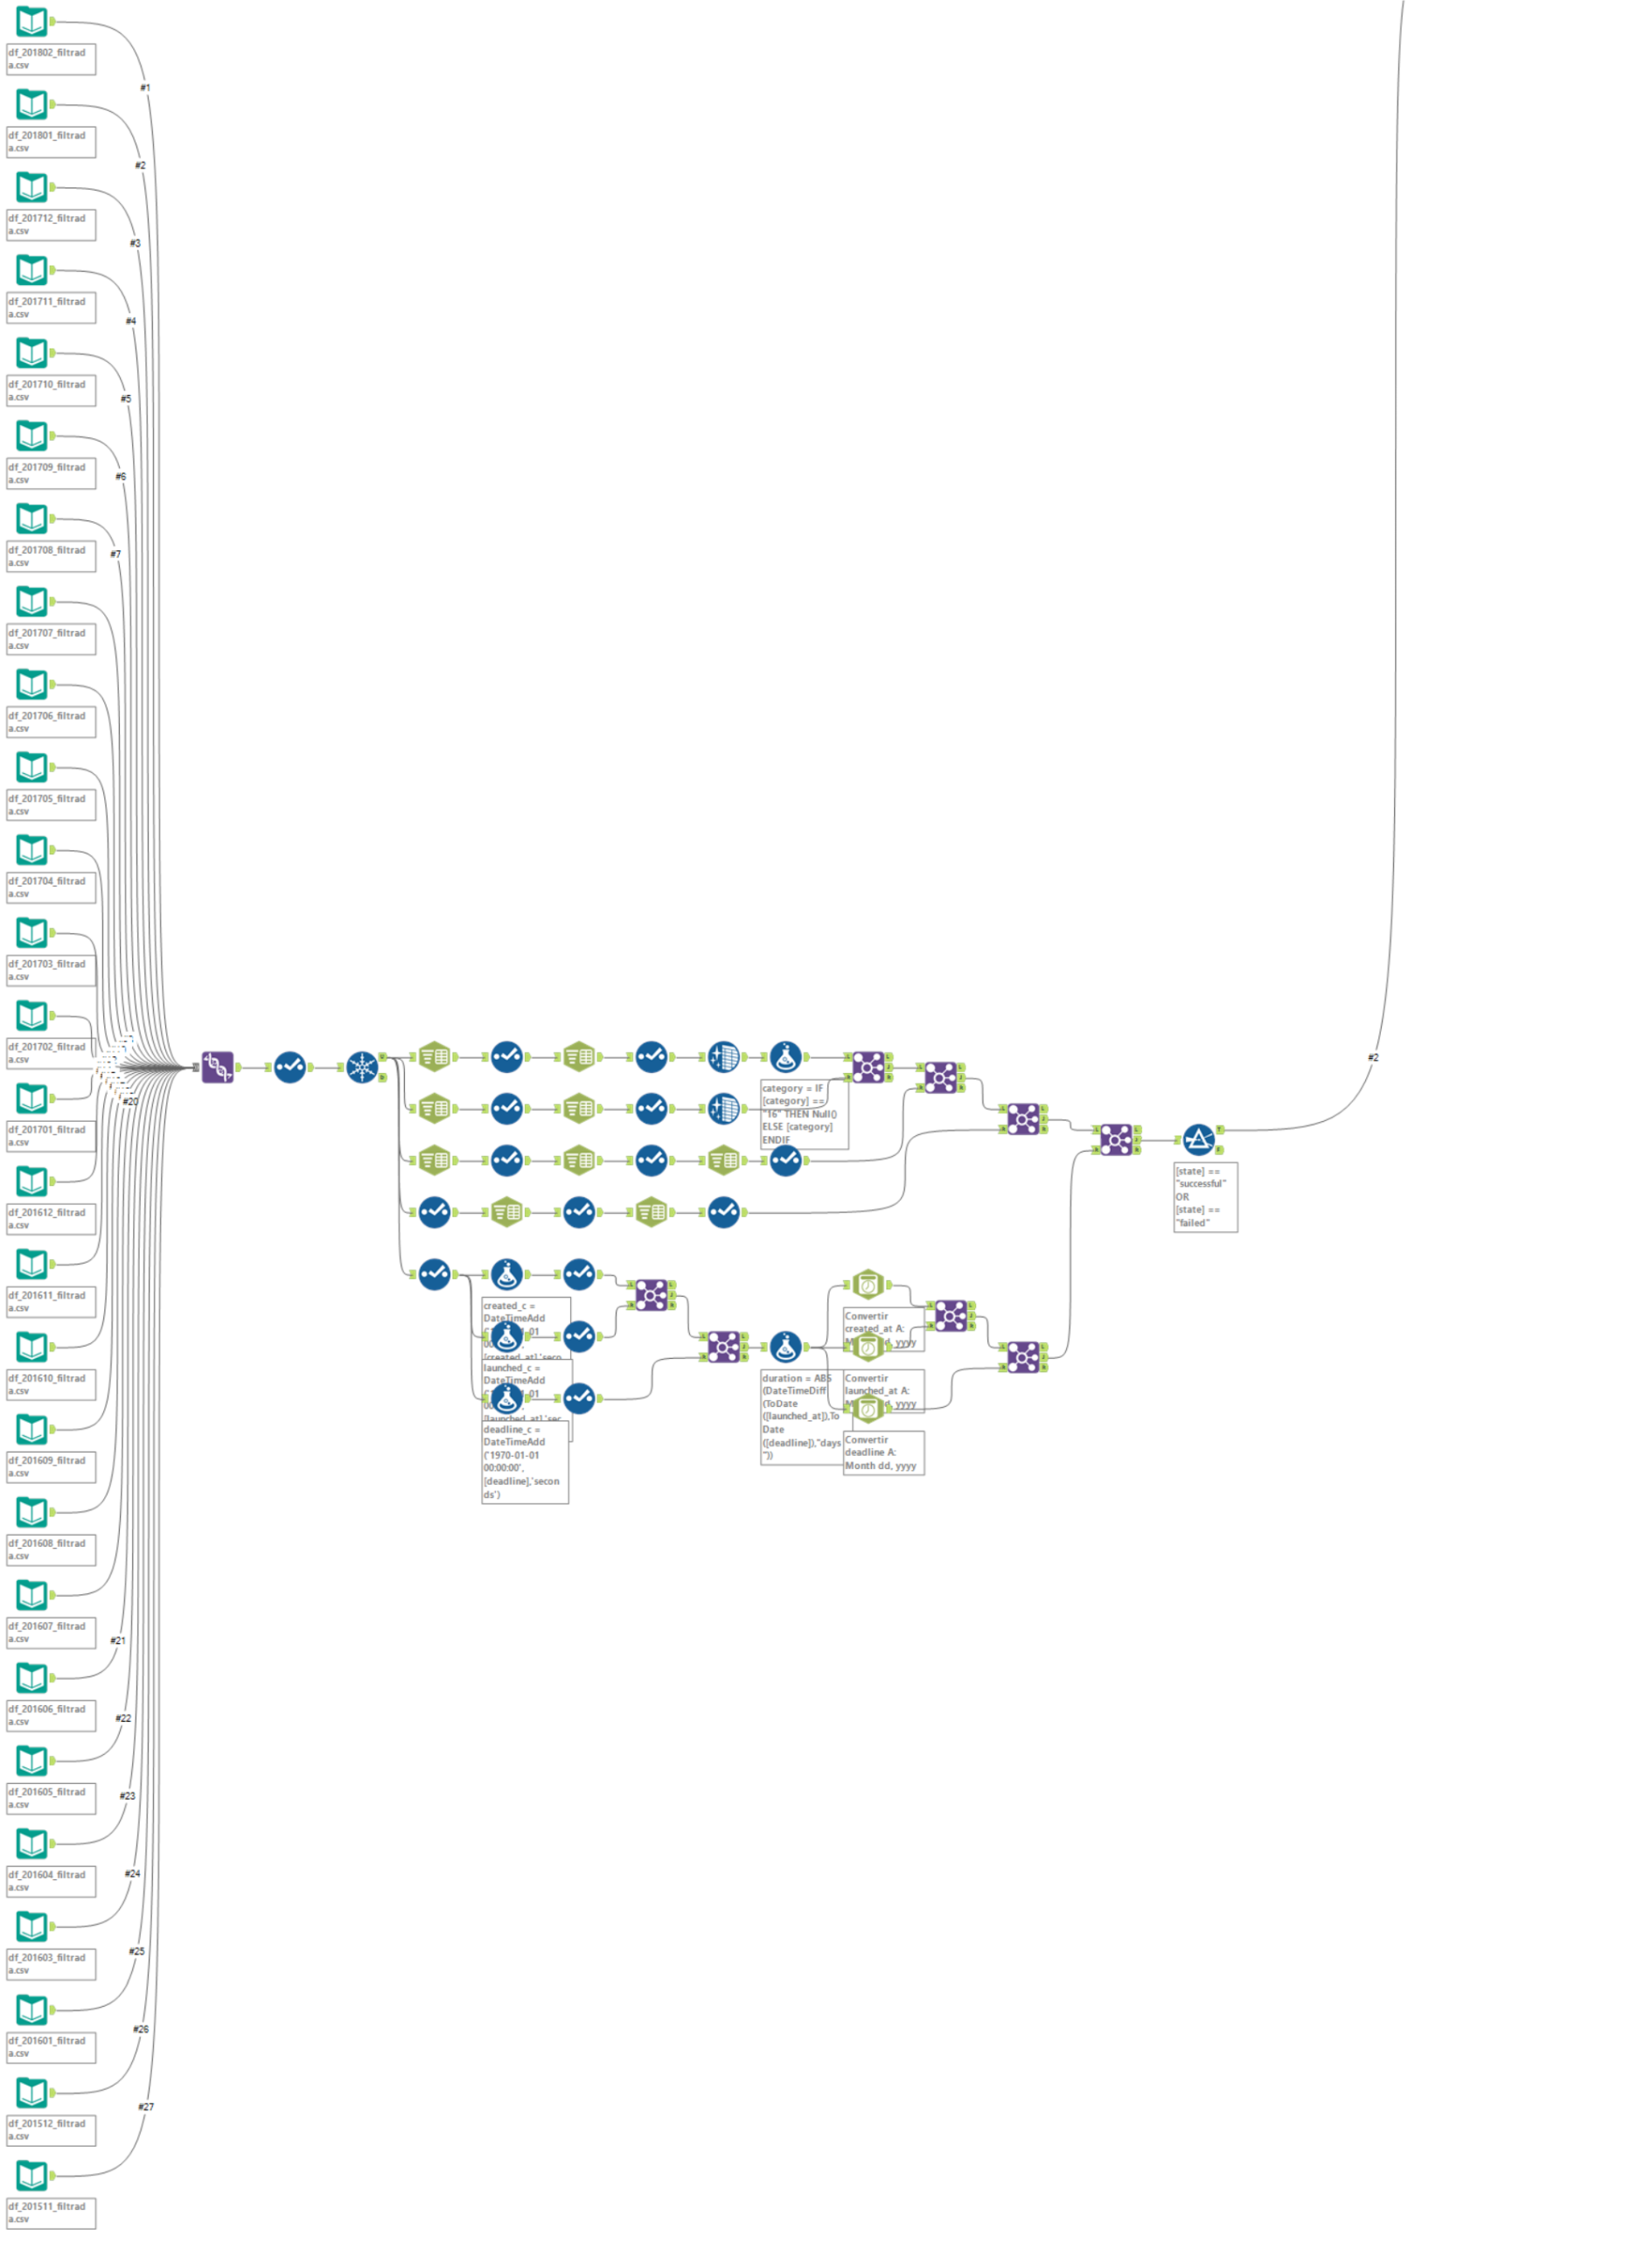
\includegraphics[width=0.7\textwidth]{4/figures/alteryx_flux_part2.png}
		\caption{Flujo de trabajo de la data final en Alteryx Designer. Fuente: Elaboración propia.}
		\label{4:fig4}
	\end{center}
\end{figure}

El flujo comienza con la carga de los datos de entrada, los cuales son los 45 archivos separados por coma por cada captura mensual desde noviembre del 2015 hasta agosto del 2019. Luego, se realizaron dos uniones en vez de una sola, esto debido a que, a partir de marzo del 2018, algunas de las variables y valores de estas son diferentes a la de sus predecesoras. Sin embargo, esto no afectará al proceso más adelante ya que ambas uniones fueron juntadas por las mismas variables.

En cada una de las dos uniones, se seleccionaron las variables de la Tabla N° 3, se realizó limpieza de datos para las variables \textit{category}, \textit{location}, \textit{photo} y \textit{urls}, y se transformaron las variables numéricas en milisegundos \textit{created\_at}, \textit{launched\_at} y \textit{deadline} a variables de fecha. Esto último permitió crear la variable \textit{duration} para determinar la duración de la campaña (en días) de un proyecto calculando la diferencia entre la fecha de culminación (\textit{deadline}) y la fecha de lanzamiento (\textit{launched\_at}). Luego se excluyeron los proyectos en proceso de la variable \textit{state} para conservar los culminados, es decir, aquellos cuyo valor sea “successful” o “failed” ya que se analizarán solamente los proyectos que han sido exitosos o fracasados. Por último, la variable \textit{urls} contiene los enlaces directos de los proyectos.

El flujograma culmina con la generación de un archivo de valores separados por coma (.csv) guardado en memoria local. Posteriormente, el archivo generado fue subido a la plataforma Kaggle de manera pública (Figura \ref{4:fig5}) para que pueda ser descargada.

\begin{figure}[h]
	\begin{center}
		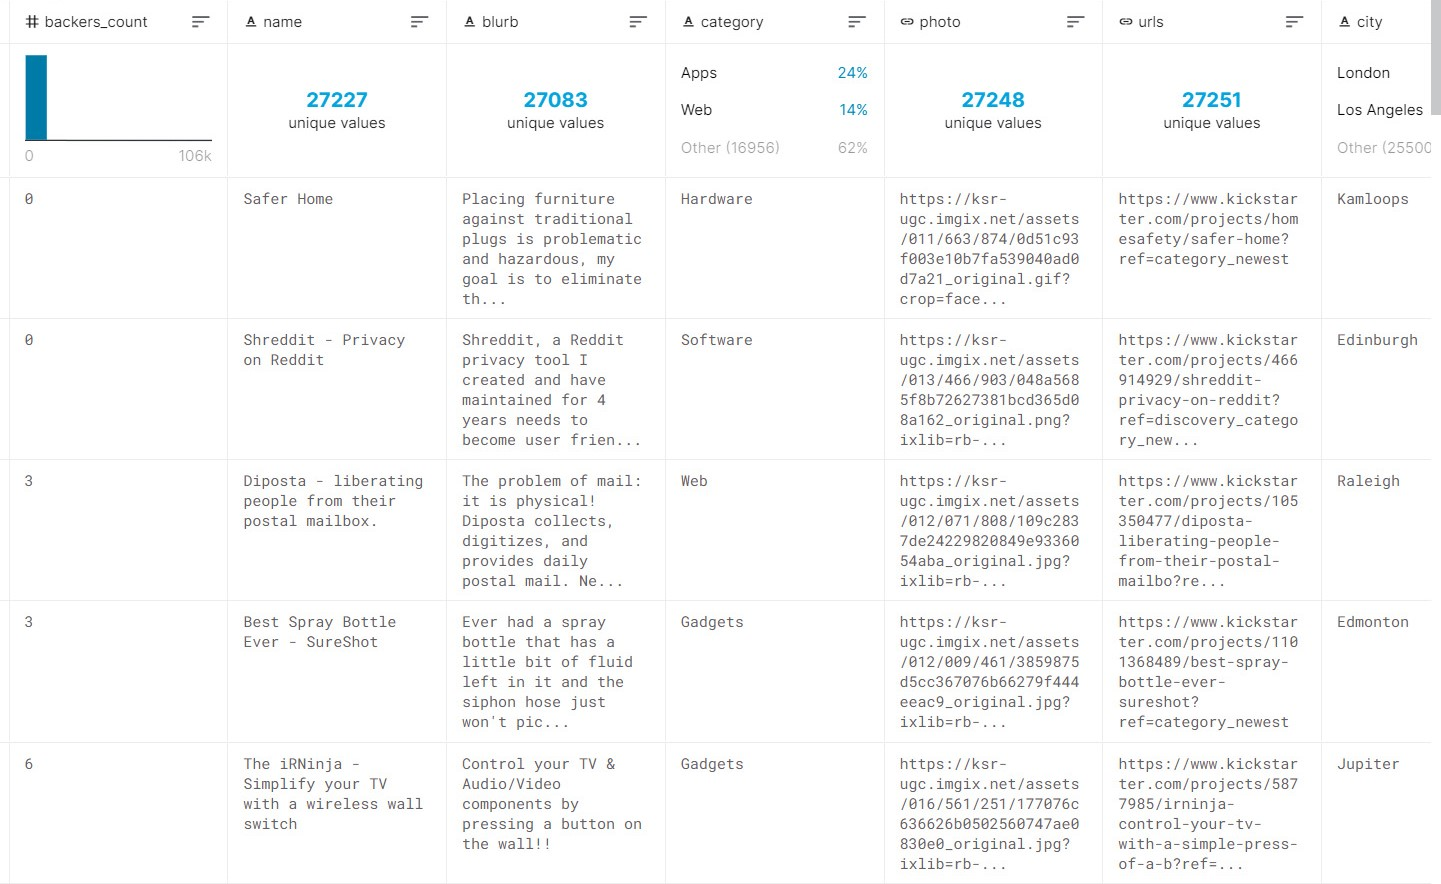
\includegraphics[width=0.8\textwidth]{4/figures/metadata_kaggle_preview.jpg}
		\caption{Visualización del archivo de metainformación subido a Kaggle. Fuente: Elaboración propia.}
		\label{4:fig5}
	\end{center}
\end{figure}

La Tabla \ref{4:table1} detalla cada variable del conjunto final, adicionando la variable \textit{pledge\_amounts} obtenida a partir de web scraping.

\begin{table}[h!]
	\centering
	\small
	\begin{tabular}{ |m{3cm}|m{10cm}|m{2cm}|  }
		\hline
		\rowcolor{bluejean}
		\Centering \color{white}{Variable}& \Centering \color{white}{Detalle}& \Centering \color{white}{Tipo de dato}\\
		\hline
		\textbf{id} & Identificador del proyecto. & number \\
		\hline
		\textbf{backers\_count} & Número de patrocinadores de la campaña del proyecto. & number \\
		\hline
		\textbf{name} &	Nombre del proyecto. &	string \\
		\hline
		\textbf{blurb} & Propaganda del proyecto. & string \\
		\hline
		\textbf{category} & Categoría (dentro de categoría principal) del proyecto. & string \\
		\hline
		\textbf{photo} & Dirección de enlace de la foto del proyecto. & string \\
		\hline
		\textbf{urls} & Dirección de la página de la campaña del proyecto. & string \\
		\hline
		\textbf{city} & Ciudad del creador del proyecto. & string \\
		\hline
		\textbf{country} & Código de país del creador del proyecto. & string \\
		\hline
		\textbf{goal} &	Monto de la meta de financiamiento del proyecto. &	float \\
		\hline
		\textbf{pledge\_amounts} & Montos disponibles para patrocinar la campaña. & string \\
		\hline
		\textbf{pledged} & Monto final patrocinado de la campaña. & float \\
		\hline
		\textbf{currency} & Divisa del monto final patrocinado. & string \\
		\hline
		\textbf{usd\_pledged} & Monto final patrocinado de la campaña (en USD). & float \\
		\hline
		\textbf{created\_at} & Fecha de creación de la campaña. & date \\
		\hline
		\textbf{launched\_at} & Fecha de lanzamiento de la campaña. & date \\
		\hline
		\textbf{deadline} & Fecha de culminación de la campaña. & date \\
		\hline
		\textbf{duration} &	Duración de la campaña (en días). &	number \\
		\hline
		\textbf{state} & Estado de financiamiento del proyecto. & string \\
		\hline
	\end{tabular}
	\caption{Diccionario de datos del conjunto final de metainformación. Fuente: Elaboración propia.}
	\label{4:table1}
\end{table}

\subsection{Descripción}
La descripción (variable \textit{description}) contiene todas las características del producto o servicio del proyecto ofrecido al público, así como otros datos importantes de la campaña. Al proveer gran cantidad de información, en los antecedentes de la investigación se confirma la relación que presenta esta observación con la performance de la campaña y, por ende, el resultado final del financiamiento del proyecto.

La variable se obtuvo utilizando web scraping en cada proyecto gracias a la variable \textit{urls}. Para ello, y como se describe en la Figura \ref{4:fig6}, se elaboró un algoritmo usando la librería BeautifulSoup que, mediante la navegación al contenido de estas páginas a través de un agente falso, se dirigió a las descripciones de los proyectos identificando las etiquetas con clase llamada “\textbf{rte\_\_content js-full-description responsive-media}” y las almacenó en un vector vacío, uniendo previamente los párrafos y eliminando caracteres especiales, para posteriormente asignarle la id correspondiente y guardarlo en un archivo de extensión .csv. En caso el algoritmo no encuentre esta clase dentro de las páginas (IndexError), el vector almacenaba un registro nulo.

\begin{figure}[!ht]
	\begin{center}
		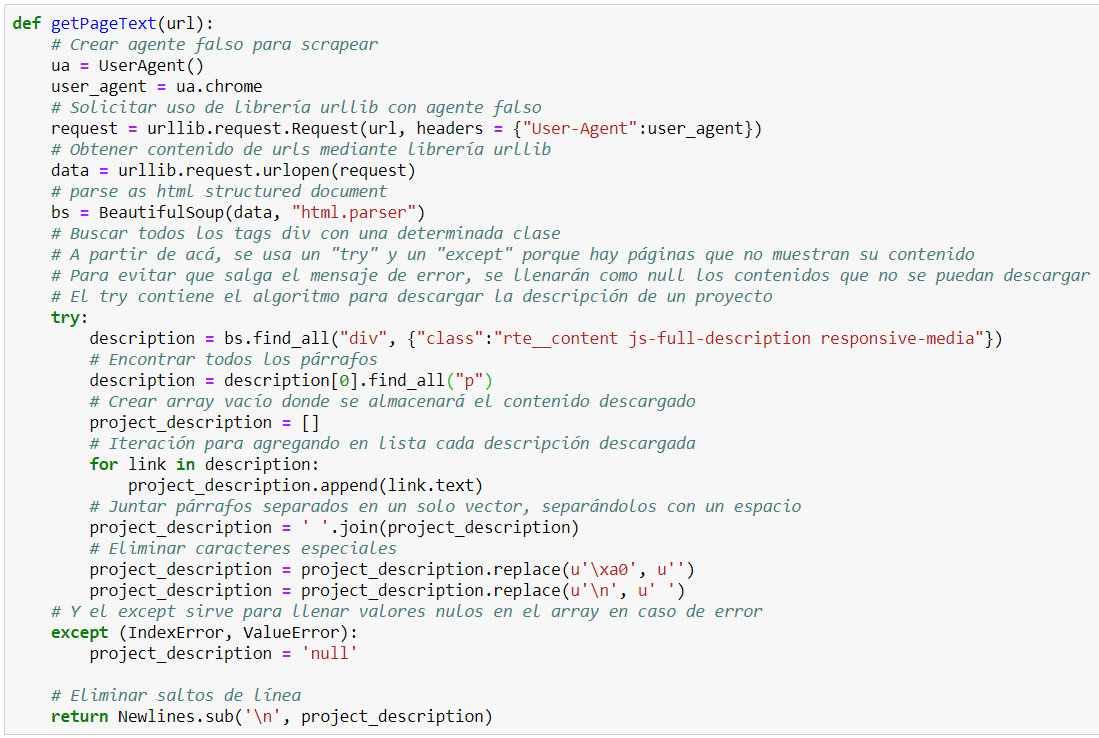
\includegraphics[width=0.8\textwidth]{4/figures/description_scraping.png}
		\caption{Función del algoritmo web scraping de la descripción de proyectos. Fuente: Elaboración propia.}
		\label{4:fig6}
	\end{center}
\end{figure}

Debido a la gran cantidad de memoria y tiempo que iba a presentar este proceso, se determinó fraccionar los 27,251 proyectos en tres partes y repetir el mismo en cada uno de ellos. El tiempo aproximado de descarga de cada fracción fue de 6 horas.

Finalmente, las tres partes fueron unidas, se reemplazaron los valores nulos por espacios en blanco y se guardó como un nuevo archivo de valores separados por coma (.csv) en código Unicode UTF-8 para la lectura de caracteres no alfabéticos.

El archivo generado fue subido a la plataforma Kaggle de manera pública (Figura \ref{4:fig7}) para que pueda ser descargada a través del API de la web.

\begin{figure}[!ht]
	\begin{center}
		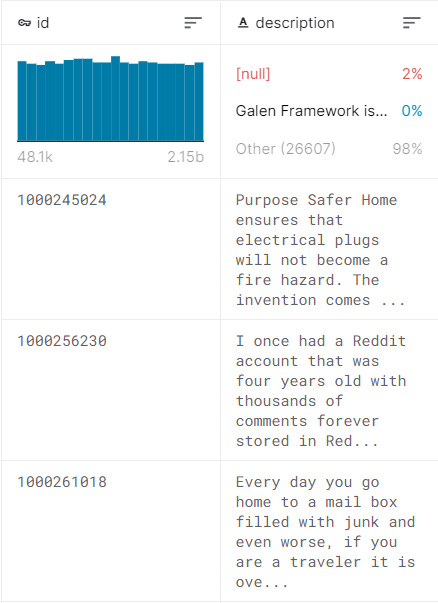
\includegraphics[width=0.4\textwidth]{4/figures/description_kaggle_preview.jpg}
		\caption{Visualización del archivo de descripción subido a Kaggle. Fuente: Elaboración propia.}
		\label{4:fig7}
	\end{center}
\end{figure}

\subsection{Comentarios}
Al igual que la descripción, los comentarios se obtuvieron utilizando la variable \textit{urls} para web scraping, pero reemplazando caracteres que contengan “\textbf{?ref=}” en adelante por “\textbf{/comments}” para redireccionarse a la sección de comentarios de cada proyecto.

Los comentarios, al ser dinámicos, no podían extraerse mediante la librería BeautifulSoup como en el caso de las descripciones, por lo que se utilizó la librería Selenium para extraerlos al iniciar una sesión desde Google Chrome, como se observa en el algoritmo de la Figura \ref{4:fig8}.

\begin{figure}[!ht]
	\begin{center}
		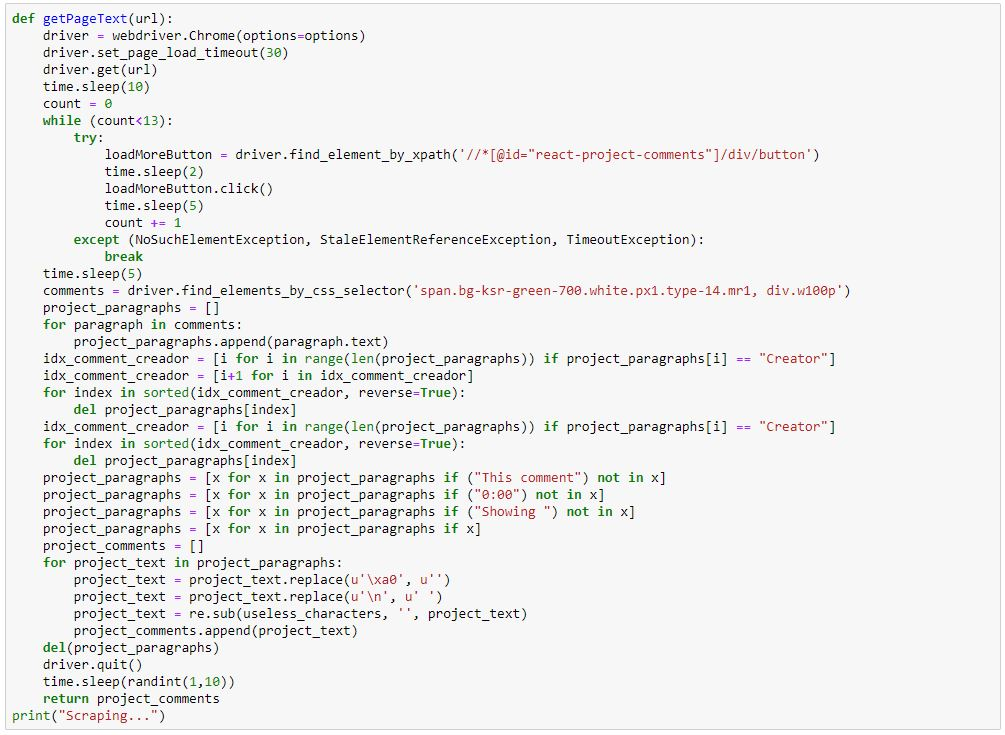
\includegraphics[width=0.8\textwidth]{4/figures/comments_scraping.jpg}
		\caption{Función del algoritmo web scraping de los comentarios. Fuente: Elaboración propia.}
		\label{4:fig8}
	\end{center}
\end{figure}

La función consiste en redireccionarse a la sección de comentarios del proyecto, esperar un máximo de 30 segundos de carga de la página, hacer clic en el botón “Load More” (Cargar más) hasta un límite de no más de 13 veces y almacenar en un vector cada comentario que no pertenezca al creador (se puede diferenciar gracias a una etiqueta en el extremo superior derecho del recuadro del comentario) de manera independiente. El siguiente paso implica la eliminación de ciertos caracteres especiales, emojis y comentarios completos de un patrocinador que no se encuentren en inglés. Finalmente, estos registros de vectores de comentarios con el id del proyecto correspondiente se almacenaron en un archivo .csv por cada fila terminada, el cual se encuentra disponible públicamente en Kaggle (Figura \ref{4:fig9}) así como los anteriores conjuntos comentados para poder ser descargados.

\begin{figure}[!ht]
	\begin{center}
		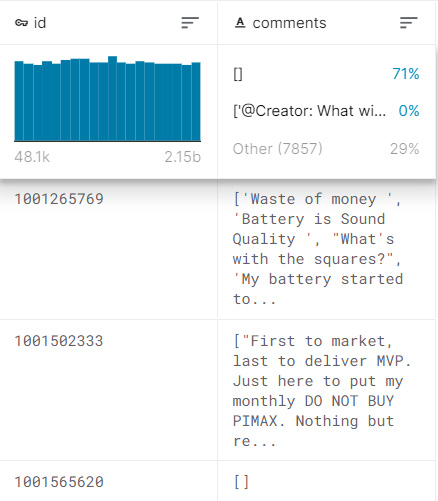
\includegraphics[width=0.4\textwidth]{4/figures/comments_kaggle_preview.jpg}
		\caption{Visualización del archivo de comentarios subido a Kaggle. Fuente: Elaboración propia.}
		\label{4:fig9}
	\end{center}
\end{figure}

Para optimizar la descarga, se crearon 8 instancias en Google Cloud (Figura \ref{4:fig10}), en donde cada una contenía dos copias del algoritmo, con la cantidad de proyectos fraccionada en 16 partes para que sean ejecutados en paralelo. Si bien el tiempo total de la consolidación de esta base de información duró aproximadamente un mes debido a percances de la conexión interna de las instancias y algunos problemas de ineficiencia de la primera versión del algoritmo, durante el transcurso dentro de este lapso de tiempo fueron solucionados hasta lograr optimizar el algoritmo de web scraping y tener el conjunto final de datos tomó menos de 48 horas.

\begin{figure}[!ht]
	\begin{center}
		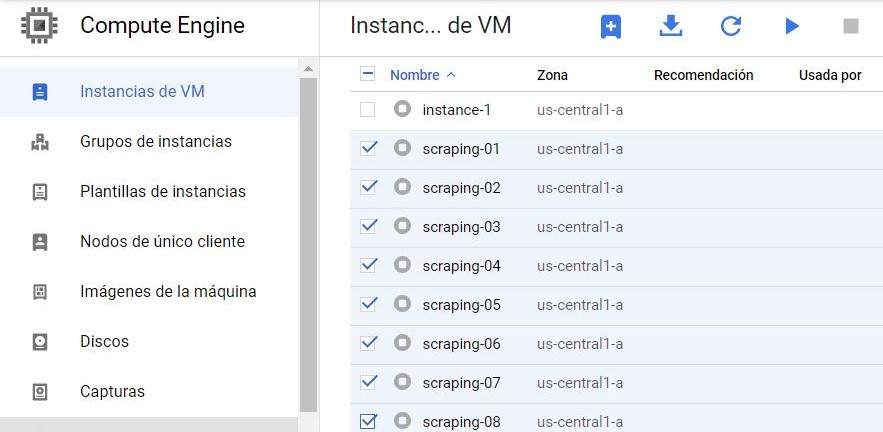
\includegraphics[width=0.7\textwidth]{4/figures/gc_instances_comments.jpg}
		\caption{Instancias lanzadas en paralelo para la extracción de comentarios. Fuente: Elaboración propia.}
		\label{4:fig10}
	\end{center}
\end{figure}

\section{Análisis Exploratorios de los datos}
Según su estado de financiamiento, los 27,251 proyectos se distribuyen mediante el gráfico de pie de la Figura \ref{4:fig11}. De esta, se observa que más del 70\% de estos fracasaron.

\begin{figure}[!ht]
	\begin{center}
		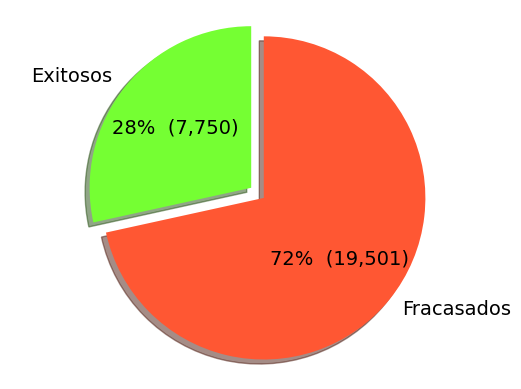
\includegraphics[width=0.55\textwidth]{4/figures/projects by state.png}
		\caption{Distribución de proyectos tecnológicos según su estado. Fuente: Elaboración propia.}
		\label{4:fig11}
	\end{center}
\end{figure}


Al visualizarlos por año (Figura \ref{4:fig12}), se puede ver que el histórico comprende entre los periodos 2009 y 2019, siendo la gran mayoría perteneciente al año 2015.

\begin{figure}[!ht]
	\begin{center}
		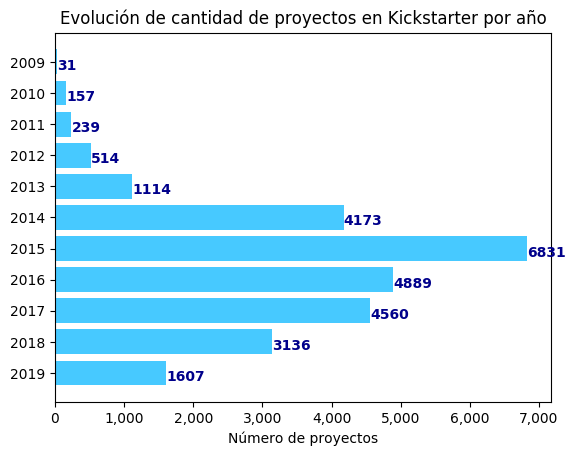
\includegraphics[width=0.7\textwidth]{4/figures/projects state by year.png}
		\caption{Evolución de cantidad de proyectos tecnológicos por año. Fuente: Elaboración propia.}
		\label{4:fig12}
	\end{center}
\end{figure}


La evolución histórica detallada por su estado se observa en la Figura \ref{4:fig13}.

\begin{figure}[!ht]
	\begin{center}
		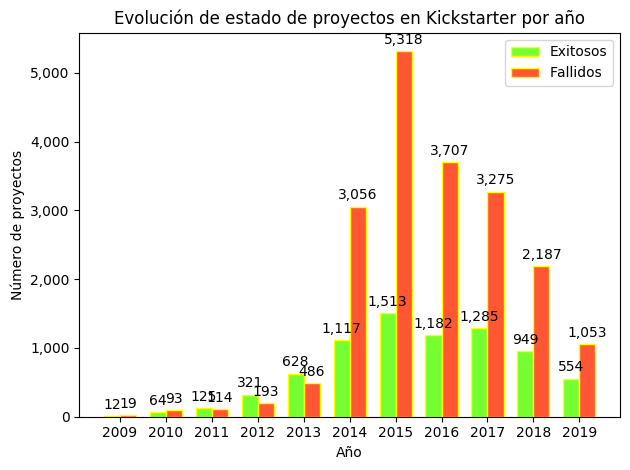
\includegraphics[width=0.7\textwidth]{4/figures/projects state evolution by year.png}
		\caption{Evolución de proyectos tecnológicos, por su estado y año. Fuente: Elaboración propia.}
		\label{4:fig13}
	\end{center}
\end{figure}

\subsection{Metainformación}
De las 19 variables de la Tabla \ref{4:table1}, y en base a los antecedentes (citar), se consideraron como potenciales variables independientes a 5 numéricas (\textit{backers\_count}, \textit{goal}, \textit{pledged}, \textit{usd\_pledged} y \textit{duration}), 3 categóricas (\textit{category}, \textit{country} y \textit{currency}) y 1 del tipo lista compuesta por números (\textit{pledge\_amounts}).

Para las variables categóricas, se realizaron gráficos de pastel para observar la distribución de sus valores. Así tenemos la Figura \ref{4:fig14} para las categorías de tecnología, Figura \ref{4:fig15} para los países (por código) y la Figura \ref{4:fig16} para las divisas del monto final patrocinado (por código). De estos tres gráficos, se observa que más de la mitad de patrocinadores provienen de los Estados Unidos (US) e invierten en dólares (USD). El segundo y tercer lugar los constituyen personas de Gran Bretaña (GB) y Canadá (CA), invirtiendo en sus monedas locales respectivas (GBP y CAD). Por el lado de las categorías, la más recurrente son de Apps, representando casi la cuarta parte del universo observado.

\begin{figure}[htbp]
	\begin{center}
		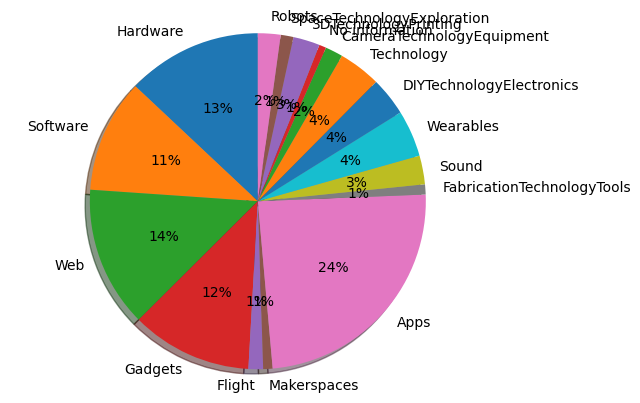
\includegraphics[width=0.65\textwidth]{4/figures/category_distribution.png}
		\caption{Distribución de categorías de tecnología. Fuente: Elaboración propia.}
		\label{4:fig14}
		
		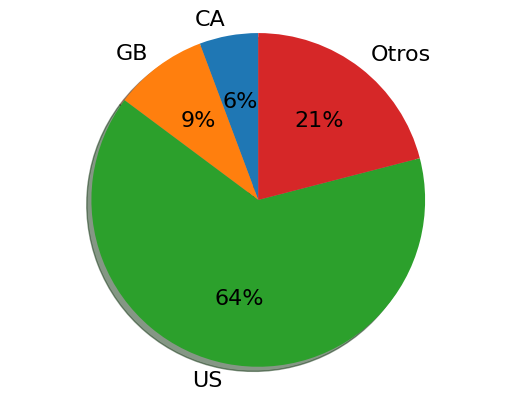
\includegraphics[width=0.55\textwidth]{4/figures/country_distribution.png}
		\caption{Distribución de países. Fuente: Elaboración propia.}
		\label{4:fig15}
		
		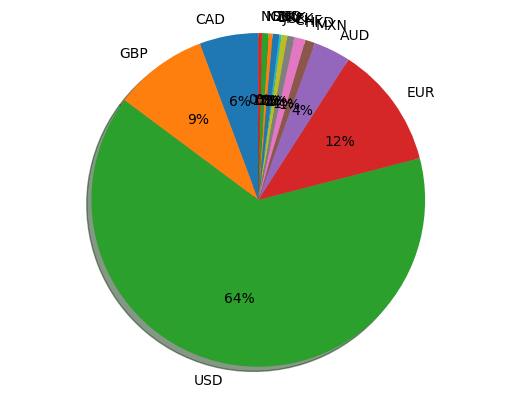
\includegraphics[width=0.55\textwidth]{4/figures/currency_distribution.png}
		\caption{Distribución de divisa del monto patrocinado. Fuente: Elaboración propia}
		\label{4:fig16}
	\end{center}
\end{figure}

Para las variables numéricas, se calcularon sus datos estadísticos con ayuda de diagramas de caja y bigote:
\begin{itemize}
	\item Número de patrocinadores de la campaña (\textit{backers\_count}):
	\begin{itemize}
		\item Rango de valores: [0; 105,857]
		\item Media: 208.710469340575
		\item Mediana: 9.487
		\item Desviación estándar: 1,179.68237749203
		\item Varianza: 1,391,650.51176525
		\begin{figure}[!ht]
			\begin{center}
				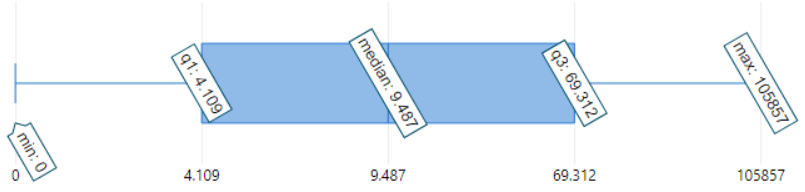
\includegraphics[width=0.7\textwidth]{4/figures/caja_bigote_backers.png}
				\caption{Diagrama de caja y bigote de patrocinadores. Fuente: Elaboración propia.}
				\label{4:fig17}
			\end{center}
		\end{figure}
	\end{itemize}
	\item Monto meta de la campaña (\textit{goal}):
	\begin{itemize}
		\item Rango de valores: [1; 100,000,000]
		\item Media: 91,263.9666162825
		\item Mediana: 15,762.614
		\item Desviación estándar: 1,259,282.1587922
		\item Varianza: 1,585,791,555,452.35
		\begin{figure}[!ht]
			\begin{center}
				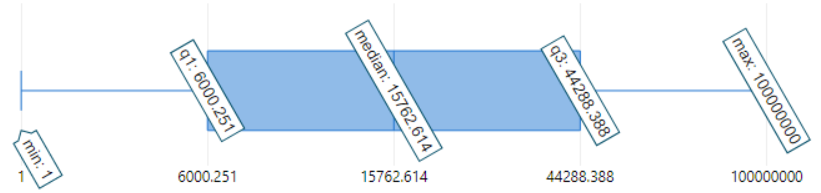
\includegraphics[width=0.7\textwidth]{4/figures/caja_bigote_goal.png}
				\caption{Diagrama de caja y bigote de meta. Fuente: Elaboración propia.}
				\label{4:fig18}
			\end{center}
		\end{figure}
	\end{itemize}
	\item Monto patrocinado al final de la campaña (\textit{pledged}):
	\begin{itemize}
		\item Rango de valores: [0; 17,406,300]
		\item Media: 34,668.5134710787
		\item Mediana: 1,382.933
		\item Desviación estándar: 226,763.900313481
		\item Varianza: 51,421,866,485.3822
		\begin{figure}[!ht]
			\begin{center}
				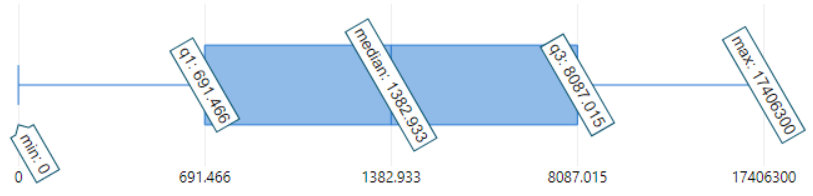
\includegraphics[width=0.7\textwidth]{4/figures/caja_bigote_pledged.png}
				\caption{Diagrama de caja y bigote de monto patrocinado. Fuente: Elaboración propia.}
				\label{4:fig19}
			\end{center}
		\end{figure}
	\end{itemize}
	\item Duración de la campaña (\textit{duration}).
	\begin{itemize}
		\item Rango de valores: [1; 92]
		\item Media: 35.4654141132436
		\item Mediana: 30
		\item Desviación estándar: 11.84570862999998
		\item Varianza: 140.320812946853
		\begin{figure}[!ht]
			\begin{center}
				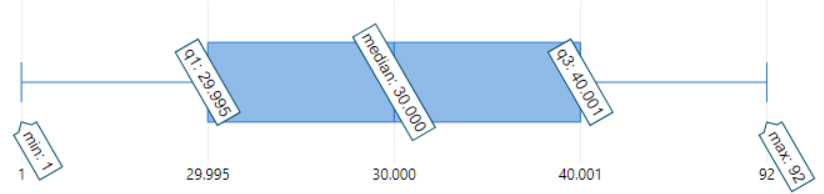
\includegraphics[width=0.7\textwidth]{4/figures/caja_bigote_duration.png}
				\caption{Diagrama de caja y bigote de duración. Fuente: Elaboración propia.}
				\label{4:fig20}
			\end{center}
		\end{figure}
	\end{itemize}
\end{itemize}

Posterior a este entendimiento de datos, se elaboró una matriz de correlaciones (Figura \ref{4:fig21}) para encontrar correlaciones entre ellas y determinar la existencia de alguna variable redundante y descartarla para no afectar el rendimiento del modelo.

\begin{figure}[!ht]
	\begin{center}
		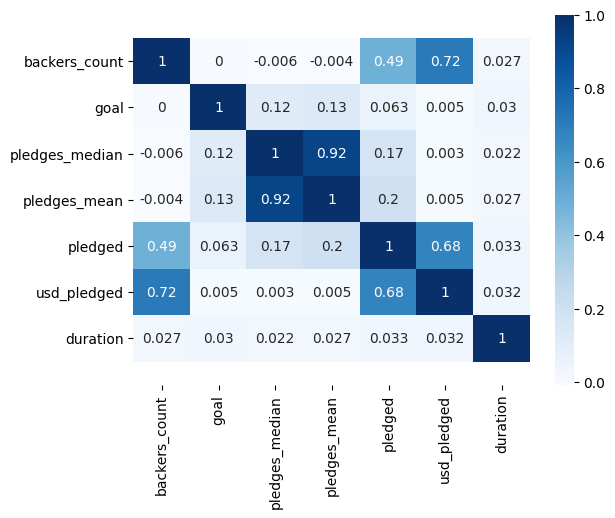
\includegraphics[width=0.65\textwidth]{4/figures/metadata correlation.png}
		\caption{Matriz de correlaciones entre variables independientes. Fuente: Elaboración propia.}
		\label{4:fig21}
	\end{center}
\end{figure}

Como se puede apreciar en la figura anterior, la variable \textit{usd\_pledged} está altamente correlacionada con las variables \textit{backers\_count} y \textit{pledged} (ambas con un aproximado de 70\%). Esto quiere decir que dicha variable no es significativa porque explicaría de manera muy similar a las otras dos.

Asimismo, si se observan los registros desde una matriz que contiene, además de gráficos de dispersión de las correlaciones, histogramas de las variables independientes como en la Figura \ref{4:fig22}, se confirma y concluye no utilizar las observaciones comentadas.

\begin{figure}[!ht]
	\begin{center}
		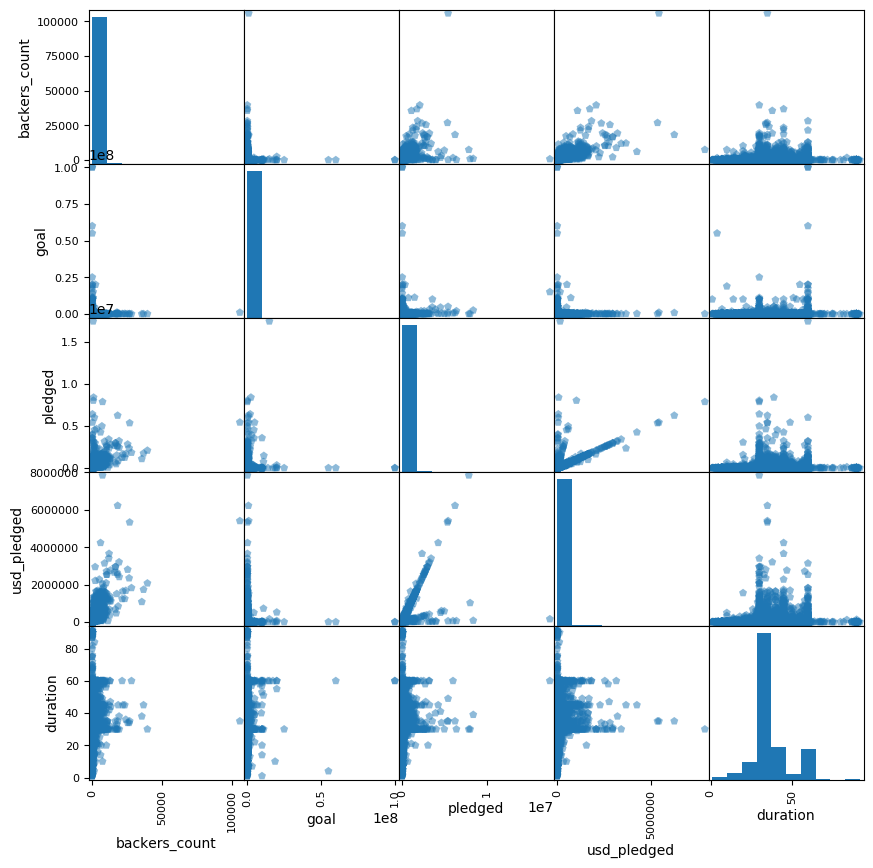
\includegraphics[width=0.80\textwidth]{4/figures/metadata cor-plot1.png}
		\caption{Gráfico de dispersión de correlaciones entre variables independientes. Fuente: Elaboración propia.}
		\label{4:fig22}
	\end{center}
\end{figure}

El mismo gráfico, segmentado por las dos clases del estado de financiamiento, se aprecia en la Figura \ref{4:fig23}.

\begin{figure}[!ht]
	\begin{center}
		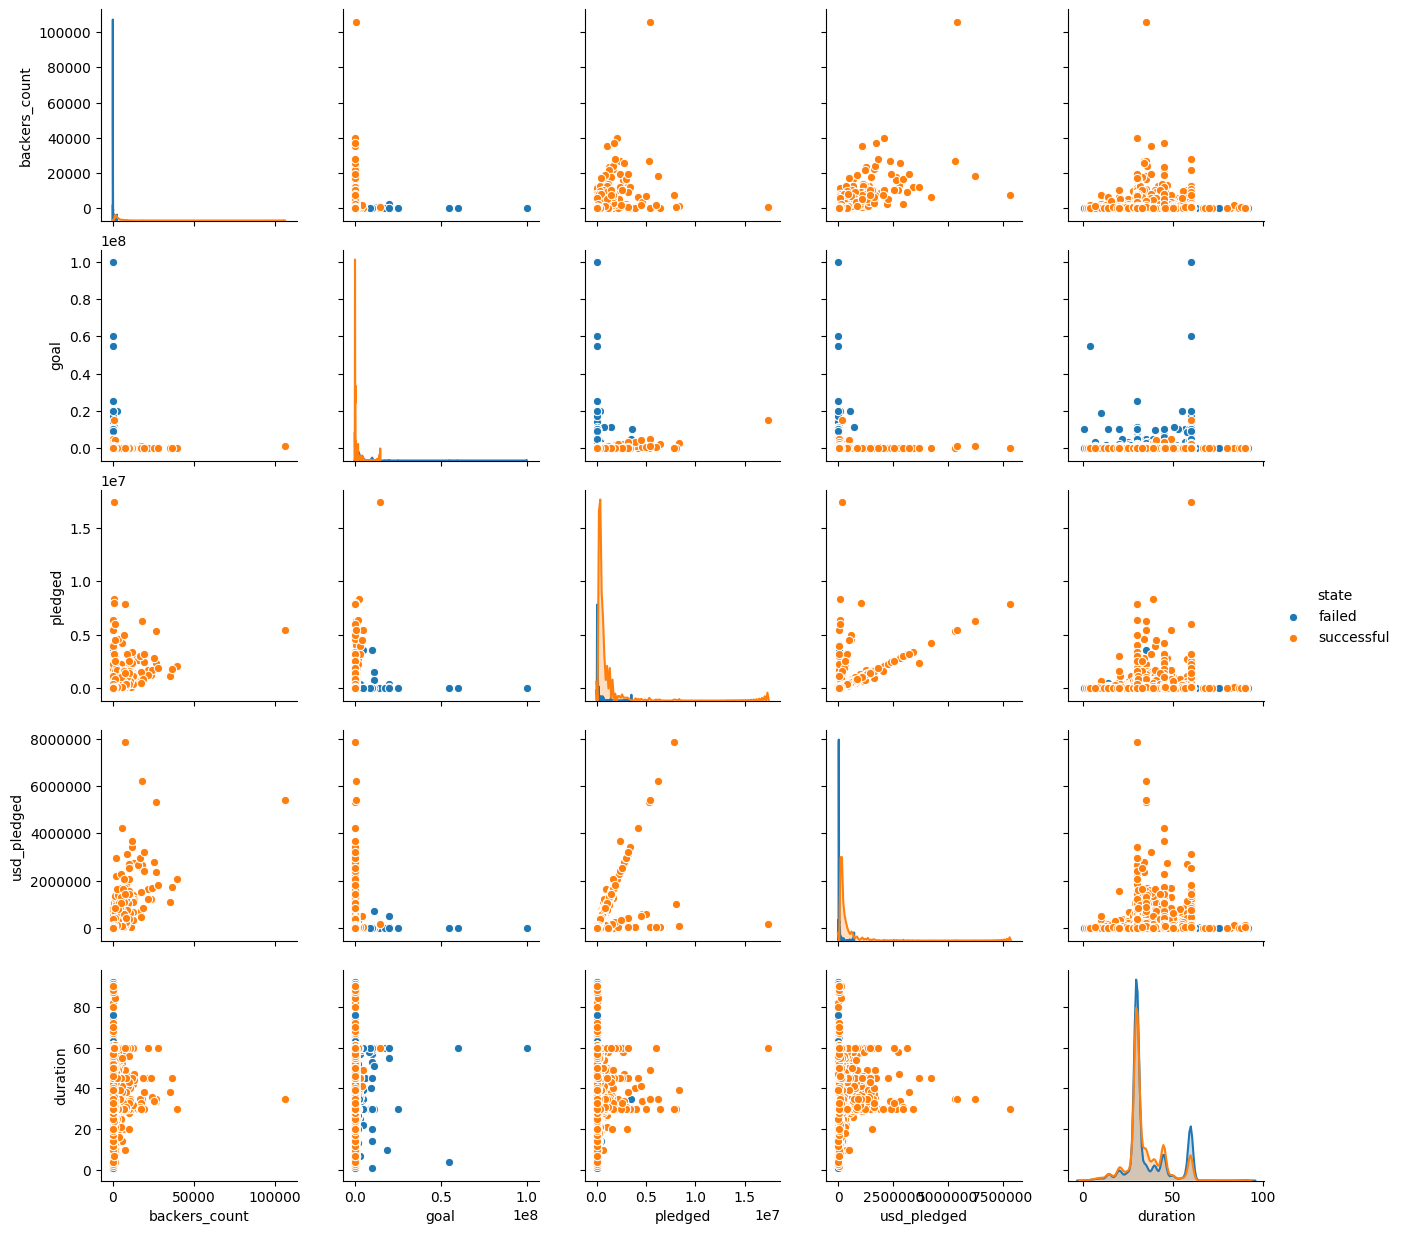
\includegraphics[width=0.80\textwidth]{4/figures/metadata cor-plot2.png}
		\caption{Gráfico alterno de dispersión de correlaciones entre variables independientes. Fuente: Elaboración propia.}
		\label{4:fig23}
	\end{center}
\end{figure}

Se concluye entonces que la variable \textit{duration} es la única que sigue una distribución normal.

\subsection{Descripción}
La descripción con mayor cantidad de palabras presenta 5,152 palabras y, a nivel total de proyectos, el vocabulario es de 165,683 palabras. La Figura \ref{4:fig24} representa la nube de palabras del contenido de cada descripción, donde las más destacadas son aquellas que aparecen con mayor frecuencia.

\begin{figure}[!ht]
	\begin{center}
		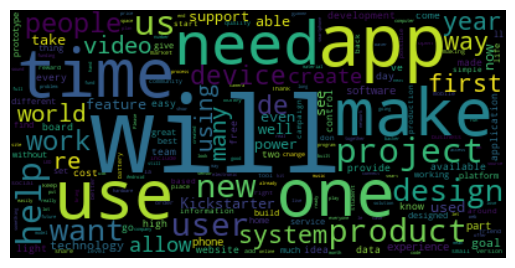
\includegraphics[width=0.7\textwidth]{4/figures/description_wordcloud_original_data.png}
		\caption{Nube de palabras de descripciones. Fuente: Elaboración propia.}
		\label{4:fig24}
	\end{center}
\end{figure}

\subsection{Comentarios}
Al analizar los proyectos exitosos y fracasados de acuerdo a la presencia de comentarios (Figura \ref{4:fig25}), se observa que hay una sólida relación entre aquellos que fracasaron y los que no cuentan con comentarios, mientras que para los proyectos exitosos, la asociación es menos contundente ya que la diferencia entre aquellos que presentan comentarios y los que no es menor.

\begin{figure}[!ht]
	\begin{center}
		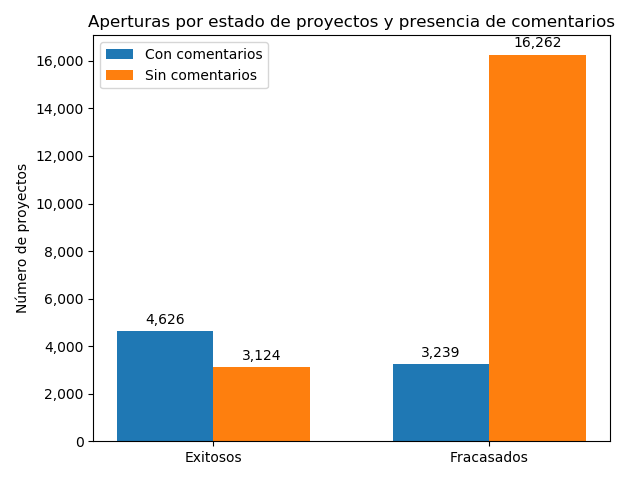
\includegraphics[width=0.7\textwidth]{4/figures/projects state by comment.png}
		\caption{Aperturas de proyectos por estado de financiamiento y presencia de comentarios. Fuente: Elaboración propia.}
		\label{4:fig25}
	\end{center}
\end{figure}

Si se repite el ejercicio del análisis anterior, ahora partiendo de los comentarios por presencia de comentarios y abiertos por su estado de financiamiento (exitosos y fracasados), se visualiza en la Figura \ref{4:fig26} una relación casi idéntica al anterior gráfico de barras.

\begin{figure}[!ht]
	\begin{center}
		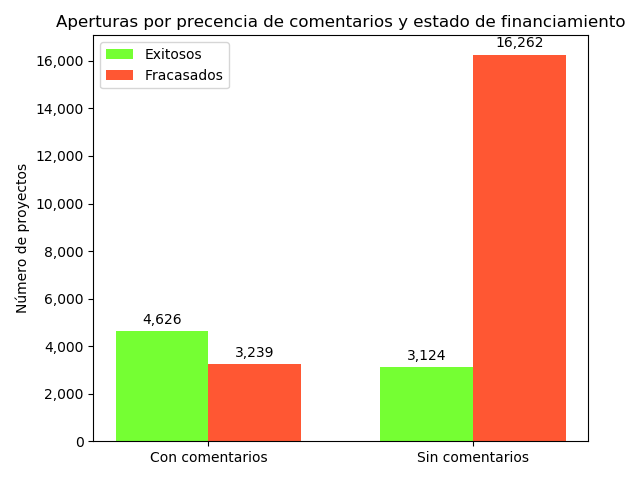
\includegraphics[width=0.7\textwidth]{4/figures/projects comment by state.png}
		\caption{Aperturas de proyectos por presencia de comentarios y estado de financiamiento. Fuente: Elaboración propia.}
		\label{4:fig26}
	\end{center}
\end{figure}

Por último, del universo de proyectos tecnológicos que presentan comentarios, los más de 4 mil proyectos exitosos contienen casi la totalidad de comentarios registrados (97\%), representando más de 475 mil como se aprecia en la Figura \ref{4:fig27}. Estos datos confirma la correlación existe entre la presencia de un volumen considerable de comentarios y su éxito de financiación.

\begin{figure}[!ht]
	\begin{center}
		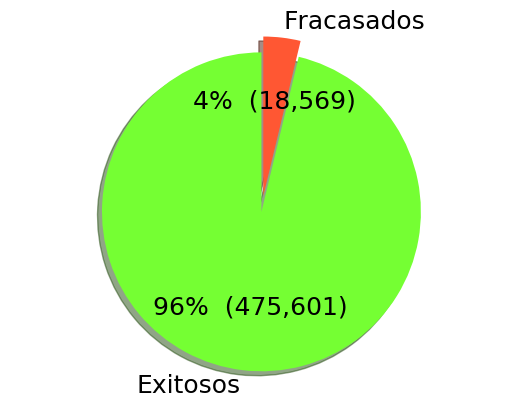
\includegraphics[width=0.8\textwidth]{4/figures/total comments by projects state.png}
		\caption{Distribución de comentarios en proyectos exitosos y fracasados. Fuente: Elaboración propia.}
		\label{4:fig27}
	\end{center}
\end{figure}

Respecto al contenido, en las Figura \ref{4:fig28} y Figura \ref{4:fig29} se ilustran las nubes de palabras de agrupadas en unidades y/o parejas más frecuentes, respectivamente.

\begin{figure}[htbp]
	\begin{center}
		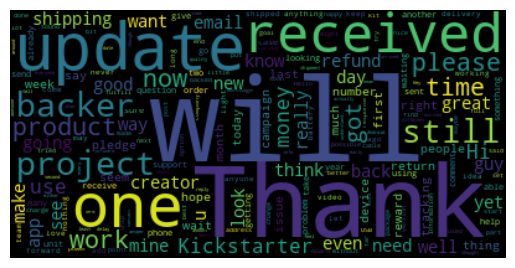
\includegraphics[width=0.70\textwidth]{4/figures/comments_wordcloud_wordunit.png}
		\caption{Nube de palabras de comentarios por unidades más frecuentes. Fuente: Elaboración propia.}
		\label{4:fig28}
		
		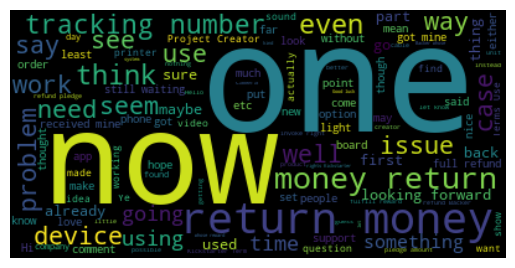
\includegraphics[width=0.70\textwidth]{4/figures/comments_wordcloud_wordcouple.png}
		\caption{Nube de palabras de comentarios por unidades o parejas más frecuentes. Fuente: Elaboración propia.}
		\label{4:fig29}
	\end{center}
\end{figure}

\section{Pre-procesamiento de los conjuntos de datos}

\subsection{Metainformación}
De acuerdo al autor (citar), se consideran 7 variables adicionales basadas en la mediana (\textit{pledges\_median}), promedio (\textit{pledges\_mean}), valor máximo (\textit{pledges\_max}), valor mínimo (\textit{pledges\_min}), variación estándar (\textit{pledges\_std}), cantidad (\textit{pledges\_num}) y completitud (\textit{completeness}) del monto prometido. La nueva matriz de correlación se observa en la Figura \ref{4:fig30}.

\begin{figure}[!ht]
	\begin{center}
		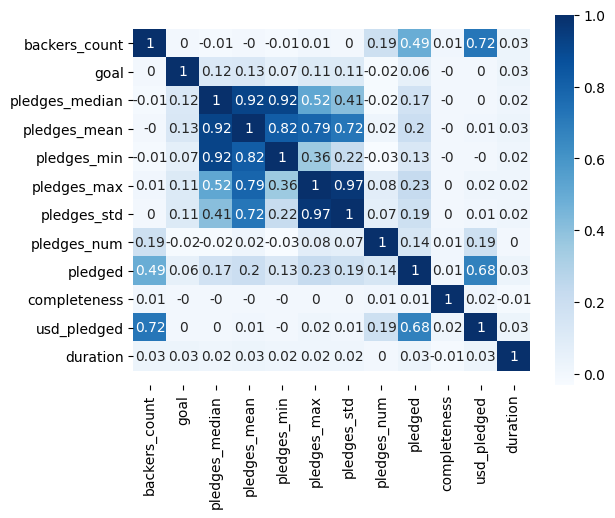
\includegraphics[width=0.8\textwidth]{4/figures/metadata correlation v2.png}
		\caption{Matriz de correlaciones entre variables independientes considerando adicionales. Fuente: Elaboración propia.}
		\label{4:fig30}
	\end{center}
\end{figure}

Como se puede observar en esta nueva matriz, el promedio presenta una alta correlación con el valor mínimo, valor máximo y la variación estándar del monto prometido. De igual manera, esta última presenta una correlación cerca a la unidad con el valor máximo. Por último, también se observa alta correlación entre el monto prometido y su conversión a dólares.

La selección de variables se considera bajo la regla de una correlación máxima de 0.30 (citar). Bajo esta norma, aquellas que cumplen son \textit{goal}, \textit{pledges\_num}, \textit{completeness} y \textit{duration}. Para conservar la mayor cantidad posible de variables, se contabilizan las variables correlacionadas con cada una de las restantes. Así por ejemplo, de acuerdo a la figura anterior, tanto \textit{pledges\_median}, \textit{pledges\_mean} y \textit{pledges\_max} sobrepasan el límite de la regla al ser tomadas en cuenta con otras 4; \textit{pledges\_min} y \textit{pledges\_std} con 3; y \textit{pledged} y \textit{usd\_pledged} con 2.

\subsection{Descripción}
De acuerdo al autor (citar), para poder entrenar un modelo de clasificación binaria basado en texto, se debe pre-procesar siguiendo el flujograma de Figura \ref{4:fig31}. Se remueven las contracciones, caracteres especiales, enlaces externos y contenidos en otros idiomas. Este resultado será tokenizado a palabras individuales con la intención de eliminar palabras de parada en inglés, lematizar las restantes y finalmente juntarlas en una lista, separadas por su proyecto correspondiente.

\begin{figure}[!ht]
	\begin{center}
		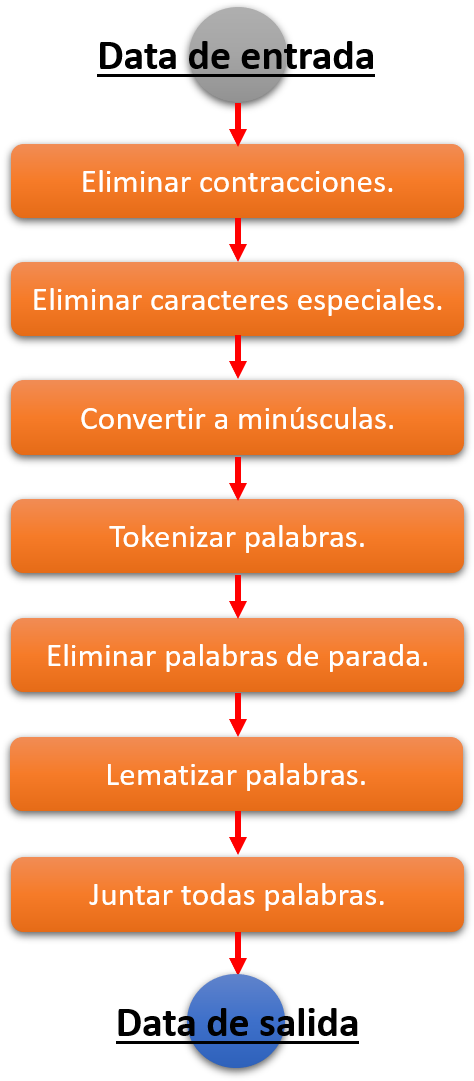
\includegraphics[width=0.35\textwidth]{4/figures/description_data_clean.png}
		\caption{Flujograma de limpieza de conjunto de datos de descripciones. Fuente: Elaboración propia.}
		\label{4:fig31}
	\end{center}
\end{figure}

Para el presente trabajo, se omitió el paso de lematización ya que según el antecedente (citar) y corroborando con los experimentos, los resultados fueron más favorables sin el anterior mencionado. Con el pre-procesamiento detallado en el párrafo anterior, la descripción de mayor longitud pasó a presentar 3,671 palabras y a nivel general de proyectos, el nuevo vocabulario tuvo 165,526 palabras.

Las nubes de palabras reflejan las palabras más frecuente dentro de un conjunto de datos. La Figura \ref{4:fig32} representa aquellas palabras que más aparecen en las descripciones de proyectos de tecnología en Kickstarter.

\begin{figure}[!ht]
	\begin{center}
		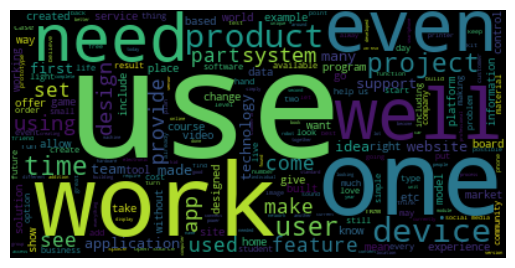
\includegraphics[width=0.7\textwidth]{4/figures/description_wordcloud.png}
		\caption{Nube de palabras de descripciones posterior al pre-procesamiento. Fuente: Elaboración propia.}
		\label{4:fig32}
	\end{center}
\end{figure}

\subsection{Comentarios}
La base de datos de comentarios está conformada por un proyecto asignado a un conjunto de comentarios de patrocinadores, separados entre sí. Antes de realizar el pre-procesamiento, se agregó un término aleatorio no relacionado con las temáticas para rellenar aquellos proyectos sin comentarios: "kuwagatabaizan".

El siguiente paso fue separar cada comentario de un mismo proyecto, manteniendo el id y estado de financiamiento correspondiente, es decir, existirán registros duplicados por la columna \textit{id}. Así, la proporción original de las etiquetas de la variable dependiente, el estado de financiamiento, será ahora de 91\% de proyectos exitosos (341,943) y 9\% fracasados (32,777).

Finalmente, se removieron caracteres especiales, espacios múltiples, signos de puntuación y números. La nueva nube de palabras se presenta en la Figura \ref{4:fig33}.

\begin{figure}[!ht]
	\begin{center}
		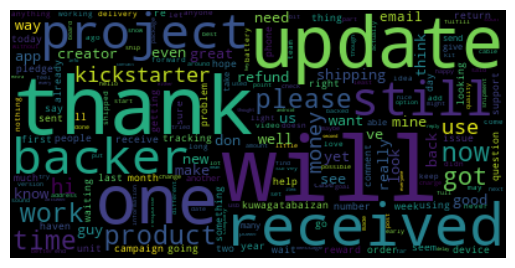
\includegraphics[width=0.7\textwidth]{4/figures/comments_wordcloud_processed.png}
		\caption{Nube de palabras de comentarios posterior al pre-procesamiento. Fuente: Elaboración propia.}
		\label{4:fig33}
	\end{center}
\end{figure}


\section{Creación de los modelos predictivos}
Una vez generado las variables independiente (observación o conjunto de observaciones, X) y dependiente (etiquetas del estado de financiamiento, Y), cada uno es separado en subconjuntos de entrenamiento y prueba, con una proporción de 80\% y 20\% respectivamente según el autor (citar) y asignándose un valor fijo de aleatoriedad. Asimismo, dentro de los parámetros de separación, se establece el argumento de estratificación según la variable Y dentro de la función train\_test\_split, de la siguiente manera:

\begin{lstlisting}[language=Python]
train_test_split(X, Y, test_size = 0.20, stratify = Y, random_state=0)
\end{lstlisting}

Antes de crear los modelos correspondientes, y después de definir los valores de entrada y parámetros (las subsecciones que se detallarán a continuación), se asigna una semilla inicial con un valor fijado por el usuario con el fin de evitar resultados aleatorios para futuras iteraciones. Se establece, además, una ruta local en donde se almacena cada punto de control basado en la mejora de la pérdida del subconjunto de validación con respecto a su iteración anterior. En caso de un estancamiento de esta última durante 10 épocas, es decir, si el valor de la pérdida no decrementa, el modelo dejará de entrenar. A esta regla se le añade la reducción de la tasa de aprendizaje luego de 5 épocas en caso el valor de la exactitud del subconjunto de validación no refleje un incremento. El objetivo de estas condiciones es evitar el sobreajuste en los modelos.

Por último, es importante asignar un peso distinto para cada una de las dos clases de la variable dependiente \textit{status}. Con el fin de evitar un mal entrenamiento, los pesos de ambas clases se balancean y se almacenan en un diccionario con su etiqueta correspondiente.

\subsection{Metainformación}
Con las entradas listas para los parámetros, se diseñó el modelo de descripciones basada en un Perceptrón Multicapa (MLP por sus siglas en inglés) bajo la arquitectura de la Figura \ref{4:fig34}. La cantidad de épocas fue de 100 y el número de lotes fue de 32.

\begin{figure}[!ht]
	\begin{center}
		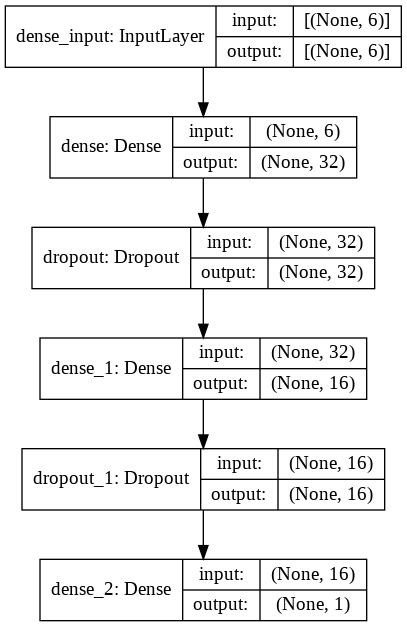
\includegraphics[width=0.40\textwidth]{4/figures/model_mlp_metadata.png}
		\caption{Arquitectura de modelo MLP para la metadata. Fuente: Elaboración propia.}
		\label{4:fig34}
	\end{center}
\end{figure}

\subsection{Descripción}
Para crear la capa de incrustación de palabras, se usa la función \textit{Tokenizer} de la librería \textbf{tensorflow.keras.preprocessing.text}, creando una función para originar un diccionario de palabras a índice al subconjunto de entrenamiento, asignándose a cada una un código. La función creada asimismo permite colocar un valor (en este caso, el término \textit{<OOV>}) a aquellos términos no entrenados y serán parte de la data de prueba (Figura \ref{4:fig35}). A continuación, los arreglos de estos textos codificados son rellenados con ceros a la derecha, hasta uniformizar con la longitud de la descripción más larga, ya que todas presentan distintos tamaños (Figura \ref{4:fig36}).

\begin{figure}[htbp]
	\begin{center}
		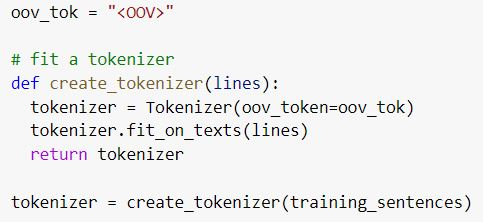
\includegraphics[width=0.50\textwidth]{4/figures/description_tokenizer_function.jpg}
		\caption{Función de tokenización de palabras de descripciones. Fuente: Elaboración propia.}
		\label{4:fig35}
		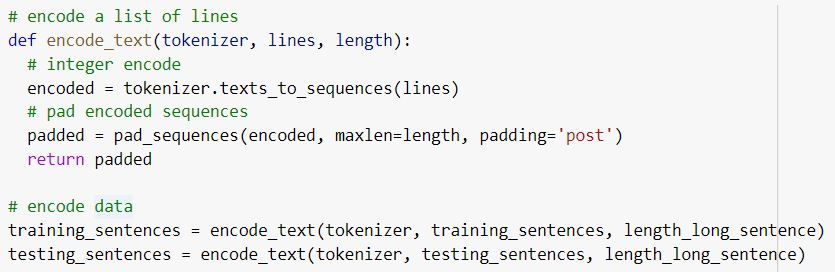
\includegraphics[width=0.80\textwidth]{4/figures/description_encoder_function.jpg}
		\caption{Función de codificación de palabras y rellenado de arreglos. Fuente: Elaboración propia.}
		\label{4:fig36}
	\end{center}
\end{figure}

Una vez obtenido el vocabulario de palabras únicas y asignado el tamaño de cada arreglo (en este caso, se asignó el de la descripción de mayor longitud), se procedió a elaborar la matriz de características usando incrustaciones de GloVe (Figura \ref{4:fig37}), un algoritmo de aprendizaje no supervisado para obtener representaciones vectoriales de palabras \parencite{gl_pennington_glove}. Para la presente investigación, se seleccionó la opción más usada, GloVe pre-entrenado con 6 billones de tokens, vocabulario de más de 400 mil palabras de Wikipedia (2014) y Gigaword (5ta edición) de la Universidad de Pensilvania, y matriz de 100 columnas, donde cada una contendrá las incrustaciones de palabras GloVe para las palabras del corpus \parencite{tec_malik2019pythonnlp}.

\begin{figure}[!ht]
	\begin{center}
		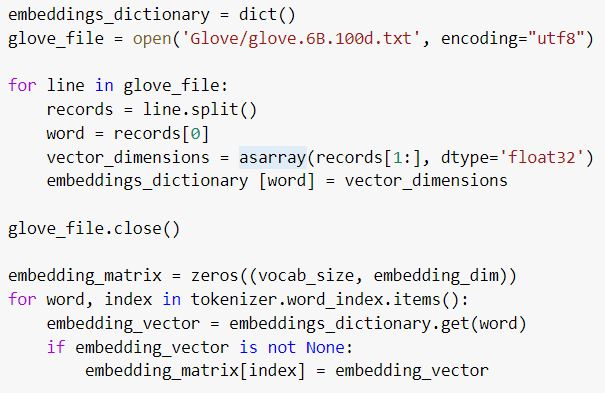
\includegraphics[width=0.60\textwidth]{4/figures/description_glove.jpg}
		\caption{Elaboración de matriz de incrustaciones de palabras. Fuente: Elaboración propia.}
		\label{4:fig37}
	\end{center}
\end{figure}

Con las entradas listas para los parámetros, se diseñó el modelo de descripciones basada en una Red Neuronal Convolucional (CNN por sus siglas en inglés) bajo la arquitectura de la Figura \ref{4:fig38}. La cantidad de épocas fue de 100 y el número de lotes fue de 128.

\begin{figure}[!ht]
	\begin{center}
		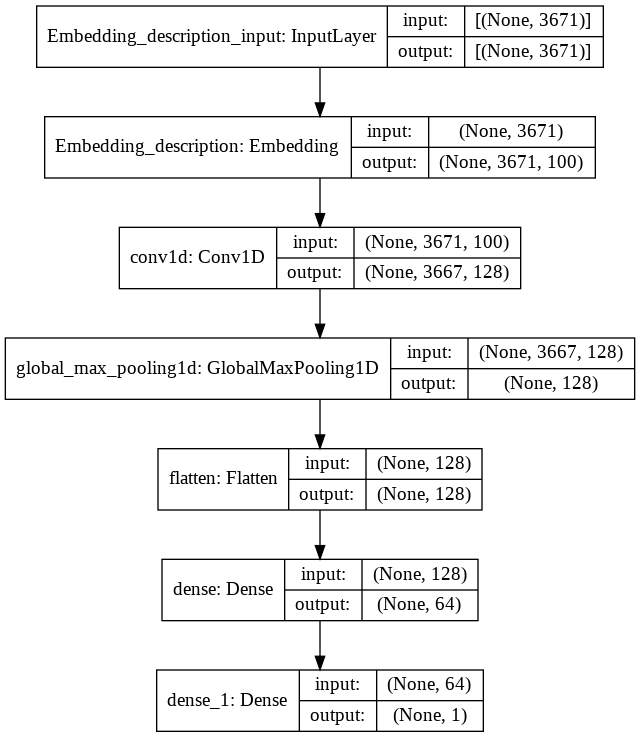
\includegraphics[width=0.60\textwidth]{4/figures/model_cnn_description.png}
		\caption{Arquitectura de modelo CNN para las descripciones. Fuente: Elaboración propia.}
		\label{4:fig38}
	\end{center}
\end{figure}

\subsection{Comentarios}